\chapter{Curve ed integrali curvilinei}

\section{Curve}

Si definiscono \textbf{Curve nello spazio} quelle applicazioni
\begin{align}
	\underline{r}(t) \, : \, [a,b] {}&\longrightarrow \mathbb{R}^3 \\
	t &\longrightarrow (x(t),y(t),z(t))
\end{align}
con 
\begin{align}
&\underline{r}(t)=(x(t),y(t),z(t)) \in C^0([a,b]) \; ; \; |r(t)|=\sqrt{x^2(t) + y^2(t) + z^2(t)} \\
&\gamma = \left\{ x(t),y(t),z(t), t\in [a,b]
\right\} \subset \mathbb{R}^3 \quad \text{sostegno della curva}
\end{align}
Se $z(t)=0$ si parla di \textbf{Curve nel piano}.

\subsection{Curve regolari}

Si dice che una curva è \textbf{regolare} se
\begin{enumerate}
	\item $\underline{r}(t)=(x(t),y(t),z(t)) \in C^1([a,b])$
	\item $\underline{r}'(t)= (x'(t),y'(t),z'(t)) \neq (0,0,0) \leftrightarrow |r'(t)|>0$
\end{enumerate}

Mentre si parla di curve \textbf{regolari a tratti} quando non c'è regolarità complessiva ma si può scomporre in sottocurve regolari.

la comodità di lavorare con le curve regolari sta, fra le altre cose, nel poter definire il \textbf{Versore tangente} alla curva:
\begin{align}
\underline{T}= \frac{(x'(t),y'(t),z'(t))}{|r'(t)|}
\end{align}
e la \textbf{Retta tangente} alla curva in un punto $(x_0,y_0,z_0)\in \gamma$:
\begin{align}
\left\{
\begin{array}{ccc}
x(t)= x_0 + x'(t_0)(t-t_0) \\
y(t)= y_0 + y'(t_0)(t-t_0) \\
z(t)= z_0 + z'(t_0)(t-t_0)
\end{array}
\right.
\end{align}

Dal punto di vista cinematico, le quantità riguardanti le curve regolari possono essere viste come:

\begin{enumerate}
	\item $\underline{r}'(t)$ è il vettore velocità
	\item $|r'(t)|$ è la velocità tangente
	\item $\underline{r}''(t)$ è il vettore accelerazione (solo se $\underline{r}(t)\in C^2$)
\end{enumerate}

\subsubsection{Esempi di curve regolari a tratti}

\begin{enumerate}
	\item $\underline{r}(t)=(t,|t|, t^3) \quad ; \quad t\in(-1,3)$
	
	Questa curva non è regolare, essendo $|t|\notin C^1((-1,3))$, ma può essere spezzata in due curve con la stessa rappresentazione negli intervalli $(-1,0)$ e $(0,3)$
	che sono invece regolari.
	
	\item $\underline{r}(t)=(t^3,t^2) \quad ; \quad t\in(-1,+1)$ 
	
	Questa non è regolar in 0, dove si annullano le derivate, ma lo è a tratti nello stesso modo della precedente 
\end{enumerate}


\subsection{Curve semplici}
	
	Si dice che una curva è \textbf{semplice} se $\underline{r}(t)$ è iniettiva in $(a,b)$ ($\underline{r}(t_1) \neq \underline{r}(t_2) \leftrightarrow t_1 \neq t_2$) o, in parole povere, non si "attorciglia". Gli estremi sono esclusi, altrimenti non si potrebbero avere curve semplici chiuse.
	
	Un esempio sono tutti i grafici di funzione su $\mathbb{R}$.
	
\subsection{Curve equivalenti}

Dati
\begin{align}
&\underline{r}(t) \, : \, [a,b] \longrightarrow \mathbb{R}^3 \\
&\tilde{\underline{r}}(\tau) \, : \, [\alpha,\beta] \longrightarrow \mathbb{R}^3
\end{align}

Due curve $(\underline{r}(t),\gamma)$ e $ (\tilde{\underline{r}}(\tau), \tilde{\gamma})$ si dicono \textbf{equivalenti} se
\begin{align}
&\exists \phi \, : \, [\alpha,\beta] \longrightarrow [a,b] \quad ; \quad \phi \in C^1([\alpha,\beta])\\
&\exists \phi^{-1} \, : \, [a,b] \longrightarrow [\alpha,\beta]  \quad ; \quad  \phi^{-1} \in C^1([a,b])
\end{align}

Ovvero abbiamo un \textbf{diffeomorfismo} tale che $\underline{r}(\phi(t))=\tilde{\underline{r}}(\tau)$

Se $\phi(\tau)>0$ gli estremi delle curve saranno uguali, altrimenti saranno invertiti.

\subsection{Lunghezza di una curva}

Consideriamo la curva $\gamma$ di sostegno $[a,b]$ in figura
\begin{figure}[!htb]
	\center{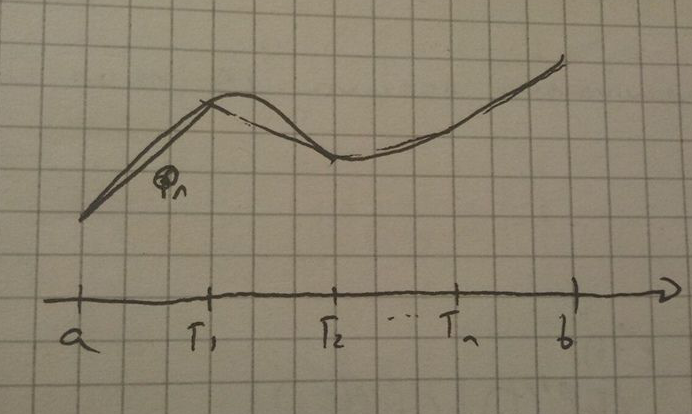
\includegraphics[width=0.5\textwidth]
		{images/curva.png}
		\caption{\label{fig:my-label}}}
\end{figure}

Una volta partizionato il sostegno in n infinitesime parti ed  individuata una spezzata poligonale $p(t)$ inscritta in $\gamma$ possiamo definire la lunghezza di $\gamma$ come
\begin{align}
lung(\gamma) = \underset{\gamma}{sup}|lung(p)|
\end{align}

Ma c'è un problema: chi ci dice che questa quantità è finita? Nessuno.

Diciamo allora che una curva è \textbf{rettificabile} se la sua lunghezza è finita.

Questa definizione è però troppo vaga per essere di utilità operativa, enunciamo quindi senza dimostrazione ("Sono pagine di conti che a noi non interessano" [cit. Lanzara]) il seguente \textbf{Teorema}:

\bigskip

\textit{Se una curva è regolare o regolare a tratti allora è rettificabile, e si avrà}
\begin{align}
lung(\gamma)=\int_{a}^{b} dt \, |r'(t)|= \int_{a}^{b} dt \, \sqrt{(x'(t))^2 + (y'(t))^2 + (z'(t))^2}
\end{align}

\textbf{Nota:} Per le curve regolari a tratti avremo $lung(\gamma)=\sum_{i=1}^{n}lung(\gamma_n)$

\bigskip

\subsubsection{Esempio: Elica Cilindrica}

$\underline{r}(t)=(R\cos(t), R\sin(t), ct) \quad; \quad t\in[0,2\pi] \, , R>0 \, c>0$

Notiamo come la curva sia regolare, essendo tutte le componenti di classe quantomeno $C^1([0,2\pi])$ ed essendo $|r'(t)|\neq (0,0,0) \; t\in(0,2\pi)$ essendo $c>0$

Avremo allora 
\bigskip

$lung(\gamma)=\int_{0}^{2\pi} dt \, \sqrt{R^2 + c^2}= 2\pi\sqrt{R^2 + c^2}$

\newpage

\subsubsection{Forma cartesiana}

Sia $y=f(x)\in C^1([a,b]) \; ; \; x\in[a,b]$, possiamo scrivere
\begin{align}
\underline{r}(t)=\left\{
\begin{array}{cc}
x=t \quad \;\,\\
y=f(t)
\end{array}
\right. \implies
lung(l)= \int_{a}^{b} dt \, \sqrt{1+ (f'(t))^2}
\end{align}

Che può però risultare scomoda, come vediamo nel seguente esempio:
\begin{align}
{}&y=f(x)=x^2 \; x\in [0,1] \implies f'(x)=2x \; f(x)\in C^1([0,1]) \\ 
&lung(l)= \int_{0}^{1} dx \, \sqrt{1+4x^2} \rightarrow \left\{
\begin{array}{cc}
t=2x \\
dt=2dx
\end{array}
\right. \rightarrow \frac{1}{2}\int_{0}^{2} dt \, \sqrt{1+t^2}
\end{align}
Facendo la sostituzione
\begin{align}
{}&t= \sinh(y)\\
&dt= \cosh(y)dy \\
&t \in [0,2] \rightarrow y \in [0,\overline{y}]
\end{align}
Avremo
\begin{align}
lung(l) {}&= \frac{1}{2} \int_{0}^{\overline{y}} dy \, \cosh(y)\sqrt{1 + \sinh^2(y)}= \nonumber \\
&=\frac{1}{2} \int_{0}^{\overline{y}} dy \, \cosh(y)\sqrt{\cosh^2(y)}= \nonumber \\
&= \frac{1}{2} \int_{0}^{\overline{y}} dy \, \cosh^2(y)= \nonumber \\
&= \frac{1}{4} \int_{0}^{\overline{y}} dy \, [1+\cosh(2y)]= \nonumber \\
&= \frac{1}{4} \left(\overline{y} + \frac{1}{2}\sinh(2\overline{y})\right)
\end{align}

\subsubsection{Lunghezze di curve equivalenti}

Supponiamo di avere due curve equivalenti $(\underline{r},\gamma)$ e $(\tilde{\underline{r}},\tilde{\gamma})$.

Dimostriamo come abbiano la stessa lunghezza:
\begin{align}
&lung(\gamma)= \int_{a}^{b} dt \, |r'(t)|=\int_{\phi^{-1}(a)}^{\phi^{-1}(b)} d\tau \, \phi'(\tau)|r'(	\phi(\tau))| \\
&lung(\tilde{\gamma})= \int_{\alpha}^{\beta} d\tau \, |\tilde{r}'(\tau)| \\
& \tilde{r}'(\tau)= \frac{d}{d\tau} \tilde{r}(\tau) = \frac{d}{d\tau} r(\phi(\tau))=r'(\phi(\tau))
\phi'(\tau)
\end{align}
Da cui ci troviamo con due casi:
\begin{enumerate}
	\item $\phi'(\tau)>0$
	
	In questo caso punti di inizio e fine coincidiono e si ha direttamente che $lung(\gamma)=lung(\tilde{\gamma})$
	
	\item $\phi'(\tau)<0$
	
	In questo caso si hanno i punti invertiti, ma tanto $|\phi'|=-\phi'$ e si ha
	\begin{align}
	lung(\gamma){}&=\int_{\beta}^{\alpha} d\tau |r'(\phi(\tau))|(-\phi'(\tau))=\int_{\alpha}^{\beta} d\tau |r'(\phi(\tau))|\phi'(\tau)= \nonumber \\
	&=lung(\tilde{\gamma})
	\end{align}
\end{enumerate}

\newpage

\subsection{Ascissa curvilinea}

Data una curva $\gamma$ con $r(t)\in[a,b]$ definiamo la funzione che calcola la lunghezza lungo la curva come
\begin{align}
{}&s(t)=\int_{a}^{t} d\tau \, |r'(\tau)| \quad ; \quad s(t) \, : \, [a,b] \longrightarrow [0,L=lung(\gamma)]\\
&s(a)=0 \; , \; s(b)=L \\
&s(t)>0 \quad \forall t \in [a,b]\\
&s(t)\in C^1([a,b]) \quad s'(t)=|r'(t)|>0
\end{align}

Dall'ultima propietà segue che $s(t)$ è anche invertibile, e si può definire l'inversa
\begin{align}
t(s) \, : \, [0,L]\longrightarrow[a,b]
\end{align}

Cosa succede se $s(t)$ e $t(s)$ rappresentano curve equivalenti?

Avremo due curve equivalenti $(r(t),\gamma)$ e $(\tilde{r}(s),\tilde{\gamma})$, con
\begin{align}
\tilde{\underline{r}}(s)=\underline{r}(t(s)) \quad ; \quad s \in [0,L]
\end{align}
E in questo caso $s$ prende il nome di \textbf{ascissa curvilinea}, la cui utilità giace nel fatto che utilizzandola il vettore tangente si normalizza, diventando versore:
\begin{align}
\frac{d}{ds}\tilde{\underline{r}}(s)= \frac{d}{ds}\underline{r}(t(s))= \frac{\partial}{\partial t}\underline{r}(t) \frac{dL}{ds}= \frac{\underline{r}'(t)}{|s'(t)|}=\frac{\underline{r}'(t)}{|r'(t)|}
\end{align}

\subsection{Curve in forma polare}

Introduciamo le coordinate polari:
\begin{align}
{}&\left\{
\begin{array}{cc}
x=\rho \cos(\theta)\\
y=\rho \sin(\theta)
\end{array}
\right.\\
\nonumber \\
&\rho=\sqrt{x^2 + y^2} \geq 0 \quad ;\quad \rho=0\leftrightarrow (x,y)=(0,0) \\
&\theta \in [0,2\pi] \; \text{oppure} \; \theta \in [-\pi,\pi] \quad ; \quad \theta=
\left\{
\begin{array}{cc}
\arctan\left(\frac{y}{x}\right) \quad {}&\forall x \neq 0 \\
\frac{(2k+1)\pi}{2} \quad &k\in \mathbb{N} 
\end{array}
\right.
\end{align}

\begin{figure}[!htb]
	\center{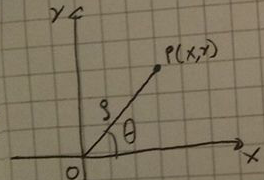
\includegraphics[width=0.5\textwidth]
		{images/coord_pol.png}
		\caption{\label{fig:my-label}}}
\end{figure}

Possiamo definire una curva in \textbf{forma polare} nel seguente modo
\begin{align}
\gamma \, : \, \underline{\rho}=\underline{\rho}(\theta)\in C^1([\theta_1,\theta_2]) \quad , \quad \theta \in [\theta_1,\theta_2]
\end{align}

Intuitivamente viene da scrivere che
\begin{align}
lung(\gamma)= \int_{\theta_1}^{\theta_2} d\theta \, |\rho'(\theta)|
\end{align}

Ma questo è \textbf{SBAGLIATISSIMO}!

\newpage

Bisogna procedere nel seguente modo:
\begin{align}
\left\{
\begin{array}{cc}
x(\theta)=\rho(\theta) \cos(\theta)\\
y(\theta)=\rho(\theta) \sin(\theta)
\end{array}
\right.
\end{align}
Da cui
\begin{align}
|r'(\theta)|^2{}&= [ \rho'(\theta) \cos(\theta) - \rho(\theta) \sin(\theta) ]^2+ [\rho'(\theta) \sin(\theta) + \rho(\theta) \cos(\theta)]^2 = \nonumber \\
&= [\rho'(\theta) \cos(\theta)]^2 - 2\rho'(\theta) \cos(\theta) \rho(\theta) \sin(\theta) + [\rho(\theta) \sin(\theta) ]^2 + \nonumber \\
&+ [\rho'(\theta) \sin(\theta)]^2 + 2\rho'(\theta) \cos(\theta) \rho(\theta) \sin(\theta) + [\rho(\theta) \cos(\theta) ]^2 = \nonumber \\
&= [\rho'(\theta)]^2 [\cos(\theta)^2 + \sin^2(\theta)] + [\rho(\theta)]^2 [\cos(\theta)^2 + \sin^2(\theta)] = \nonumber \\
&= [\rho'(\theta)]^2 + [\rho(\theta)]^2
\end{align}
Questo ci porta ad avere una quantità maggiore di zero solo in caso di curve regolari e ad avere
\begin{align}
|r'(\theta)| = \sqrt{[\rho'(\theta)]^2 + [\rho(\theta)]^2}
\end{align}
Che ci porta alla corretta espressione di lunghezza di una curva in forma polare:
\begin{align}
lung(\gamma)= \int_{\theta_1}^{\theta_2} d\theta \, \sqrt{[\rho'(\theta)]^2 + [\rho(\theta)]^2}
\end{align}

\subsection{Esempi di curve}

\subsubsection{Cicloide}

\begin{align}
\underline{r}(t)=\left\{
\begin{array}{cc}
x(t)= r \, \cdot (t-\sin(t)) \\
y(t)= r \, \cdot (1-\cos(t))
\end{array}
\right. \quad ; \quad t \in [0,2\pi]
\end{align}

Notiamo come le componenti siano ben più che di classe $C^1$ e otteniamo

\begin{align}
{}&\underline{r}'(t)=\left\{
\begin{array}{cc}
x'(t) {}&= r \, \cdot (1-\cos(t)) \\
y'(t) &= r \, \cdot \sin(t) \qquad \;\,\,
\end{array}
\right. \\
\nonumber \\
&|r'(t)|^2= r^2 \, \cdot (1 - 2\cos(t) + \cos^2(t) + \sin^2(t))=2r^2(1-\cos(t))\\
&|r'(t)|^2 >0 \quad \forall t \in (0,2\pi) \\
& |r'(t)|= \sqrt{2} \; r \, \sqrt{1-\cos(t)}
\end{align}

Da cui ricaviamo 

\begin{align}
lung(\gamma)= \sqrt{2} \; r \int_{0}^{2\pi}dt \, \sqrt{1-\cos(t)} = 2r   \int_{0}^{2\pi} dt \, \sin\left(\frac{t}{2}\right) = 8 r
\end{align}

\subsubsection{Ellittica}

\begin{align}
\left(
\frac{x}{a}
\right)^2 + \left(
\frac{y}{b}
\right)^2=1 \quad ; \quad a,b>0
\end{align}

\begin{align}
{}&\underline{r}(t)=\left\{
\begin{array}{cc}
x(t)= a \cos(t) \\
y(t)= b \sin(t)
\end{array}
\right. \quad ; \quad t \in [0,2\pi]\\
&|r'(t)|= [-a \sin(t)]^2 + [b \cos(t)]^2
\end{align}

\begin{align}
lung(\gamma) {}&= \int_{0}^{2\pi} dt \, \sqrt{[-a \sin(t)]^2 + [b \cos(t)]^2} = \nonumber \\
&= \int_{0}^{2\pi} dt \, \sqrt{a^2 [1-\cos^2(t)] + b^2 \cos^2(t)}  = \nonumber \\
&= \int_{0}^{2\pi} dt \, \sqrt{a^2 + (b^2-a^2)\cos^2(t)} = \nonumber \\
&= \int_{0}^{2\pi} dt \, \sqrt{1 + \frac{b^2-a^2}{a^2}\cos^2(t)} = \nonumber \\
&= \int_{0}^{2\pi} dt \, \sqrt{1 + e \cos^2(t)} \quad ; \quad e= \frac{b^2-a^2}{a^2} \quad \text{elliticità}
\end{align}

questi integrali non sono di facile risoluzione e o si trovano tabulati o si approssima.

\subsubsection{Cardioide (curva in forma polare)}

\begin{align}
{}&\rho(\theta)= a[1+\cos(\theta)] \quad ; \quad \theta \in [-\pi, +\pi] \, , \, a>0 \\
&\rho'(\theta)= - a \sin(\theta) \\
&\underline{r}(t)=\left\{
\begin{array}{cc}
x(t)= a[1+\cos(\theta)] \cos(t) \\
y(t)= a[1+\cos(\theta)] \sin(t)
\end{array}
\right. \quad ; \quad t \in [0,2\pi]
\end{align}

Per semplicità poniamo $a=1$ e otteniamo
\begin{align}
lung(\gamma){}&= \int_{-\pi}^{+\pi} d\theta \, \sqrt{\sin^2(\theta) + [1+\cos(\theta)]^2} = \nonumber \\
&= \int_{-\pi}^{+\pi} d\theta \, \sqrt{ 2 + 2 \cos(\theta)}= \nonumber \\
&=\sqrt{2} \int_{-\pi}^{+\pi} d\theta \, \sqrt{ 1 +  \cos(\theta)}= 2 \int_{-\pi}^{+\pi} d\theta \, \left|\cos\left(\frac{\theta}{2}\right)\right|=8
\end{align}


\subsubsection{Spirale logaritmica}
\begin{align}
{}&\rho = \Exp{\theta} \spacer \theta\in[0,2\pi]\\
&\underline{r}(\theta)=\double{x(\theta)= \Exp{\theta}\cos(\theta) }{y(\theta) = \Exp{\theta}\sin (\theta)}\\
& lung(\gamma)= \int_{0}^{2\pi}d\theta \, \sqrt{\Exp{2\theta} + \Exp{2\theta}} = \sqrt{2}\int_{0}^{2\pi}d\theta \, \Exp{\theta}= \sqrt{2}(\Exp{2\theta} -1)
\end{align}

\subsubsection{Spirale di Archimede}

\begin{align}
{}&\rho = \theta \spacer \theta\in[0,\frac{\pi}{6}]\\
&\underline{r}(\theta)=\double{x(\theta)= \theta\cos(\theta) }{y(\theta) = \theta\sin (\theta)}\\
& lung(\gamma)= \int_{0}^{\frac{\pi}{6}}d\theta \, \sqrt{1 + \theta^2} = \int_{0}^{\overline{u}}du \, \cosh^2(u) = \frac{\pi}{2} + \fracn{4}\sinh \left(\frac{\pi}{3}\right)
\end{align}

Abbiamo applicato il seguente cambio di variabile
\begin{align}
{}&\theta = \sinh(u) \implies d\theta = \cosh(u)du \\
&1 + \theta^2= 1 + \sinh^2(u) = \cosh^2(u)
\end{align}


\newpage

\section{Integrali curvilinei}


\subsection{Integrali curvilinei di I tipo (o di funzione)}

Sia una curva regolare 
\begin{align}
\gamma \, : \, \underline{r}(t)=(x(t),y(t),z(t)) \quad ; \quad t \in [a,b]
\end{align}
e sia
\begin{align}
f \, : \, A \subseteq \mathbb{R}^3 {}&\longrightarrow \mathbb{R} \\
(x,y,z) & \longrightarrow f(x,y,z)
\end{align}
quantomeno continua e tale che $(\mathbb{R}^3, ||\cdot||_3) \longrightarrow (\mathbb{R},||\cdot||)$, avremo allora
\begin{align}
\int_{\gamma} ds \, f = \int_{a}^{b} dt \, f(x(t),y(t),z(t))\sqrt{[x'(t)]^2 + [y'(t)]^2 + [z'(t)]^2}
\end{align}
Che ci rappresenta questa quantità? Possiamo dargli due interpretazioni:
\begin{enumerate}
	\item \textbf{Geometrica:}

	\begin{figure}[!htb]
		\center{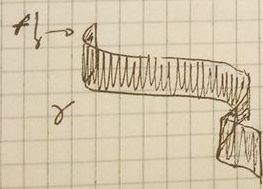
\includegraphics[width=0.5\textwidth]
			{images/int_curv.png}
			\caption{\label{fig:my-label}}}
	\end{figure}
	
	L'integrale misura il "muro" che viene "innalzato" lungo $\gamma$ da $f(x,y,z)$
	
	\item \textbf{Fisica:}

	L'integrale misura la massa di un filo di lunghezza $\gamma$ e densità $f(x,y,z)$ (ha senso se $f(x,y,z)\geq 0$)
\end{enumerate}

Per curve equivalenti $\gamma_1$ $\gamma_2$ si ha che 
\begin{align}
\int_{\gamma_1} ds \, f = \int_{\gamma_2} ds \, f
\end{align}

Con indipendenza dal verso di percorrenza. La dimostrazione di questa proprietà discende direttamente da quella della lunghezza di curve equivalenti.

\textbf{Caso particolare:} la funzione identità restituisce la lunghezza della curva!

Gli integrali curvilinei del Io tipo godono delle seguenti proprietà:

\begin{enumerate}
	\item \textbf{Linearità:
	\begin{align}
	\int_{\gamma} ds \, (\alpha f + \beta g)= \alpha\int_{\gamma} ds \, f + \beta \int_{\gamma} ds \, g
	\end{align}}

	\item \textbf{Monotonia}:
	\begin{align}
	f\leq g \implies \int_{\gamma} ds \, f \leq \int_{\gamma} ds \, g
	\end{align}
	
	\item \textbf{Teorema del modulo:}
	\begin{align}
	\left| \int_{\gamma} ds \, f \right| \leq \int_{\gamma} ds \, |f|
	\end{align}
\end{enumerate}

\newpage

\subsection{Esempi di I.C. di Io tipo}

\begin{enumerate}
	\item $\gamma \taleche x^2 +y^2 =1 \spacer x,y \geq 0 = z$ 
	\begin{align}
	{}&\underline{r}(t)= \double{x(\theta)= \cos(\theta)}{y(\theta) = \cos(\theta)}\spacer \theta \in \left[0,\frac{\pi}{2}\right] \\
	&|r'(t)|= \sqrt{\sin^2(\theta) + \cos^2(\theta)}=1 \spacer ds = |r'(t)|dt=dt\\
	&\int_{\gamma} ds (x + y -1) = \int_{0}^{\frac{\pi}{2}}d\theta ( \cos(\theta) + \sin(\theta) -1)= \dots = 2 - \frac{\pi}{2}
	\end{align}

	\item $\gamma \taleche \underline{r}(t) \triple{x(t)= \cos(t)}{y(t)= \sin(t)}{z(t)=t} \spacer t \in [0,\pi] \implies |r'(t)|= 2 \spacecomma ds = \sqrt{2}dt$
	\begin{align}
	\int_{\gamma} ds (x^2 + y^2 + z^2) {}&= \sqrt{2}\int_{0}^{\pi} dt (1 + t^2) = \sqrt{2} \left[t|_0^\pi + \left.\frac{t^3}{3}\right|_0^\pi \right] = \continue &=\sqrt{2}\left(\pi + \frac{\pi^3}{3}\right)
	\end{align}
	
\end{enumerate}

\subsection{Baricento (o centro di massa) di una curva}

Si definisce \textbf{baricentro} di una curva con densità lineare $f\geq 0$ il punto con coordinate
\begin{align}
{}&x_B=\frac{\int_{\gamma}ds \, x\cdot f}{\int_{\gamma}ds \, f} \\
&y_B=\frac{\int_{\gamma}ds \, y\cdot f}{\int_{\gamma}ds \, f} \\
&z_B=\frac{\int_{\gamma}ds \, z\cdot f}{\int_{\gamma}ds \, f}
\end{align}

\textbf{Nota bene:} non è detto che $(x_B,y_B,z_B)\in\gamma$

Vediamo in pratica di cosa si parla con l'esempio del quarto di asteroide:
\begin{align}
{}&\underline{r}(t)=\left\{
\begin{array}{cc}
x(t)=\cos^3(t)\\
y(t)=\sin^3(t)
\end{array}
\right. \quad ; \quad t\in \left[0,\frac{\pi}{2}\right]\\
&f=1 \quad \text{densità costante}\\
&|r'(t)|= 3 \sin(t)\cos(t) 
\end{align}

	\begin{figure}[!htb]
	\center{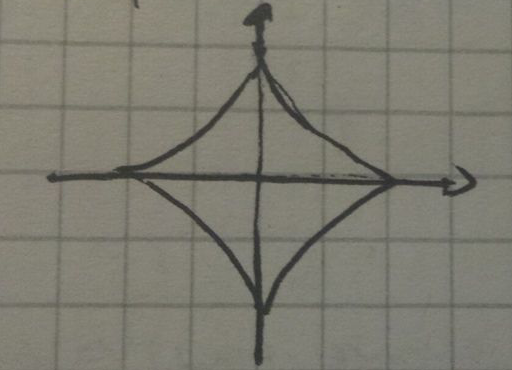
\includegraphics[width=0.4\textwidth]
		{images/asteroide.png}
		\caption{\label{fig:my-label}}}
	\end{figure}
\begin{align}
lung(\gamma){}&= \int_{\gamma}ds \, f = 3 \int_{0}^{\frac{\pi}{2}} dt \, \sin(t)\cos(t)\rightarrow \left\{
\begin{array}{cc}
u=\cos(t)\\
du=\sin(t)dt
\end{array}
\right. \rightarrow 3\int_{0}^{1} du \, u = \nonumber\\
&=\frac{3}{2}u^2|_{0}^{1}=\frac{3}{2}
\end{align}	
\begin{align}
x_B {}&= \int_{\gamma}ds \, x\cdot f = 3 \int_{0}^{\frac{\pi}{2}} dt \, \cos^3(t)\cdot \sin(t)\cos(t) = \nonumber \\
&= \int_{0}^{\frac{\pi}{2}} dt \, \cos^4(t)\sin(t) = \nonumber \\
&= - 3 \int_{1}^{0} du \, u^4 = \frac{3}{5}u^5|_{0}^{1}= \frac{3}{5} \\
\nonumber \\
y_B &= \int_{\gamma}ds \, y\cdot f= 3 \int_{0}^{\frac{\pi}{2}} dt \, \sin^3(t)\cdot \sin(t)\cos(t)=\nonumber \\
&= \dots = \nonumber \\
&= \frac{2}{5}
\end{align}
	
\subsection{Integrali curvilinei di II tipo (o di campo vettoriale)}

Prima di definirli, ci domandiamo: cos'è un campo vettoriale?

È un vettore tale che
\begin{align}
\underline{F}(x,y,z)\, : \, A \subseteq \mathbb{R}^3 {}&\longrightarrow \mathbb{R}^3 \\
(x,y,z) &\longrightarrow (F_1(x,y,z),F_2(x,y,z),F_3(x,y,z)) \nonumber
\end{align}
Le cui componenti sono quantomeno continue.

Supponiamo ora di avere $\gamma\in A$, e definiamo il \textbf{versore tangente} come
\begin{align}
\underline{T}(t)=\frac{(x'(t),y'(t),z'(t))}{\sqrt{[x'(t)]^2 + [y'(t)]^2 + [z'(t)]^2}}
\end{align}

E possiamo infine definire gli \textbf{integrali curvilinei di IIo tipo} come
\begin{align}
\int_{\gamma}ds \, \underline{F}\cdot \underline{T}
\end{align}

Questa quantità ha un significato fisico ben preciso: è il lavoro delcampo di forze $\underline{F}$ per spostare lungo $\gamma$ un corpo puntiforme. Lo indicheremo quindi con $W$.

Operativamente questa definizione è però poco utile, memori quindi di quanto fatto per gli integrali di primo tipo, e svolgendo il prodotto tra i due vettori otteniamo:
\begin{align}
W{}&=\int_{\gamma}ds \, \underline{F}\cdot \underline{T} = \nonumber \\
&= \int_{a}^{b}dt \, \left[F_1(r(t)) \frac{x'(t)}{|r'(t)|} + F_2(r(t)) \frac{y'(t)}{|r'(t)|} + F_3(r(t)) \frac{z'(t)}{|r'(t)|}
\right] |r'(t)|= \nonumber \\
&= \int_{a}^{b}dt \, \left[F_1(r(t)) x'(t) + F_2(r(t)) y'(t) + F_3(r(t)) z'(t)
\right]
\end{align}

\textbf{Nota bene:} Mentre per gli integrali di I tipo per curve equivalenti il risultato era lo stesso anche per versi opposti, in questo caso il verso di percorrenza è rilevante.

\subsubsection{Esempi di Integrali curvilinei di II tipo}

Calcoliamo ora il lavoro di una serie di campi vettoriali.

\begin{enumerate}
	\item $\underline{F}=(1,0,0)$ lungo il segmento $\underline{x_0}=(0,0,0)\longrightarrow \underline{x_1}=(1,2,3)$
	
	L'unica rappresentazione possibile per il segmento sarà:
	
	\begin{align}
		{}&\underline{r}(t)=\left\{
		\begin{array}{ccc}
			x(t) = x_0 + (x_1 - x_0)t\\
			y(t) = y_0 + (y_1 - y_0)t\\
			z(t) = z_0 + (z_1 - z_0)t 
		\end{array}
		\right. \implies
		\underline{r}(t)=\left\{
		\begin{array}{ccc}
			x(t) ={}& \, t\\
			y(t) =& 2t\\
			z(t) =& 3t 
		\end{array}
		\right. \quad ; \quad
		\underline{r}'(t)=\left\{
		\begin{array}{ccc}
			x'(t) ={}& 1\\
			y'(t) =& 2\\
			z'(t) =& 3 
		\end{array}
		\right. \nonumber \\
		\nonumber\\
		&W=\int_{0}^{1} dt \, [1\cdot 1 + 0 \cdot 2 + 0 \cdot 3]= \int_{0}^{1}dt = 1
	\end{align}
	
	\item $\underline{F}=(y \, , \, x^2 + y^2\, , \, 0)=(y\, , \, x^2 + y^2)$ 
	
	lungo l'arco di circ. $x^2 + y^2=4$ con estremi   $\underline{x}_0=(-2,0) \longrightarrow \underline{x}_1=(0,2)$
	
	\begin{align}
		{}& {x}_0=(-2,0) \longrightarrow \underline{x}_1=(0,2) \implies t_0=\pi \longrightarrow t_1=\frac{\pi}{2}\\
		&\underline{r}(t)=\left\{
		\begin{array}{cc}
			x(t)=2\cos(t) \\
			y(t)=2\sin(t)
		\end{array}
		\right. \quad ; \quad
		\underline{r}'(t)=\left\{
		\begin{array}{cc}
			x'(t)=-2\sin(t) \\
			y'(t)=+2\cos(t)
		\end{array}
		\right.
	\end{align}
	\begin{align}
		W {}&= - \int_{\frac{\pi}{2}}^{\pi} dt \, [2\sin(t)\cdot (-2\sin(t)) + 4 \cdot (2\cos(t))] = \nonumber \\
		&=4 \int_{\frac{\pi}{2}}^{\pi} dt \, [\sin(t) -2\cos(t)]= \dots = \pi + 8
	\end{align}
	
	\item \textbf{Il campo gravitazionale:} 
	$\underline{F}=\frac{Gm}{(x^2 + y^2 + z^2)^{\frac{3}{2}}}(x,y,z)$
	
	Data una generica curva $\gamma \, : \, r(t)=(x(t),y(t),z(t))$ con $t\in[a,b]$ contenuta in $A\subseteq \mathbb{R}^3 \backslash\left\{(0,0,0)\right\}$
	
	\begin{align}
		W {}&= -Gm \int_{a}^{b} dt \, \frac{1}{(x^2 + y^2 + z^2)^{\frac{3}{2}}} [x(t)x'(t) + y(t)y'(t) + z(t)z'(t)] = \nonumber \\ 
		&= -Gm \int_{a}^{b} dt \, \frac{d}{dt}\left(\frac{1}{\sqrt{x^2 + y^2 + z^2}}\right)= -Gm \int_{a}^{b} dt \, \frac{d}{dt}\left(\frac{1}{|r(t)|}\right)  = \nonumber \\ 
		&= Gm\left(\frac{1}{|r(b)|} - \frac{1}{|r(a)|}\right)
	\end{align}
	Notiamo l'indipendenza dal percorso ma non dai punti di inizio e fine.
\end{enumerate}
